
\chapterimage{MathCover.png} % Chapter heading image

\chapter{Wastewater Math Review}\index{Wastewater Math Review}

\section{Unit Conversions}\index{Unit Conversions}


% \begin{enumerate}
% \definecolor{shadecolor}{RGB}{200, 200, 240}
% \begin{snugshade*}
%\section{Units and Unit Conversion}\index{Units and Unit Conversion}
% 	\item \noindent\textsc{Units and Unit Conversion}
% \end{snugshade*}

For converting one measurement unit to another.

Step 1:  \texthl{Make sure the original unit is for the same measurement as the converted (desired) unit.}  So if the original unit is for area, say in ft$^2$ the converted unit should be another area unit such as in$^2$ or acre but it cannot be gallons as gallon is a unit of volume.

Step 2: Write down the conversion formula as:

$Quantity \enspace in \enspace converted \enspace unit = Quantity \enspace (\cancel{Original \enspace Unit}) *   Conversion  \enspace Factor \enspace  \dfrac{Conversion \enspace unit}{\cancel{Original \enspace unit}}$


\begin{table}[h!]

\begin{center}
    \begin{tabular}{ | p{4cm} |p{8cm}|}
    \hline
    
    
Length  & inches, ft, miles\\
\hline 
Area  & ft$^2$, acres \\
\hline 
Volume & ft$^3$, gallons, acres-ft.\\
\hline 
Density & weight per volume, lbs/ft$^3$, lbs/gallon\\
\hline 
Flow & ft$^3$/min, MGD, acres-ft/day\\
\hline 

	

    \end{tabular}
 \caption{Common units in wastewater calculations}	
    \end{center}

    \end{table}

%Powers of Ten
%
%\begin{center}
%    
%   
%    \begin{tabular}{ | c | p{4cm} | c |p{8cm}|}
%    \hline
%
%%\hline
%%\multicolumn{4}{|c|}{\textbf{ESSAYS}} \\
%%\hline
%%\thead{A Head} & \thead{A Second \\ Head} & \thead{A Third \\ Head} \\
%%\hline%
%
%$10^{12}$ & 1,000,000,000,000 & Tera & Like in tera byte drive - trillion\\
%\hline 
%$10^{9}$ & 1,000,000,000 & Giga & Like in giga byte data - billion\\
%\hline
%$10^{6}$ & 1,000,000 & Mega & Like in mega bytes or megawatts - million\\
%\hline 
%$10^{3}$ & 1,000 & Kilo & Like in kilogram \\
%\hline 
%$10^{0}$ & 1 &  & \\
%\hline 
%$10^{-3}$ & 0.001 & milli & Like in millimeter - thousandth of a meter\\
%\hline 
%$10^{-6}$ & 0.000001 & micro & Like in microgram - millionth of a gram \\
%\hline 
%$10^{-9}$ & 0.000000001 & nano & Like in nanometer - billionth of a meter\\
%\hline 
%
%
%    \end{tabular}
%    
%    \end{center}





\subsection{Example Problems}\index{Example Problems}
\begin{enumerate}
\item Convert 1000 $ft^3$ to cu. yards\\

$1000 \cancel{ft^3}*\dfrac{cu.yards}{27\cancel{ft^3}} = 37 cu.yards$
\vspace{6pt}
\item Convert 10 gallons/min to $ft^3$/hr\\

$\dfrac{10 \cancel{gallons}}{\cancel{min}}*  \dfrac{ft^3}{7.48 \cancel{gallons}}  * \dfrac{60 \cancel{min}}{hr}   = \dfrac{80.2ft^3}{hr}$

\vspace{6pt}
\item Convert 100,000 $ft^3$ to acre-ft.\\
$100,000 \cancel{ft^3} * \dfrac{acre-ft}{43,560 \cancel{ft^2-ft}} =  2.3 acre-ft$\\
\textbf{Note:} From the conversion table: acre = 43,560 $ft^2$\\
Thus, acre-ft  = 43,560 $ft^2$-ft\\
\end{enumerate}


\section{Area and Volume Calculations}
\begin{table}[h!]
\begin{center}
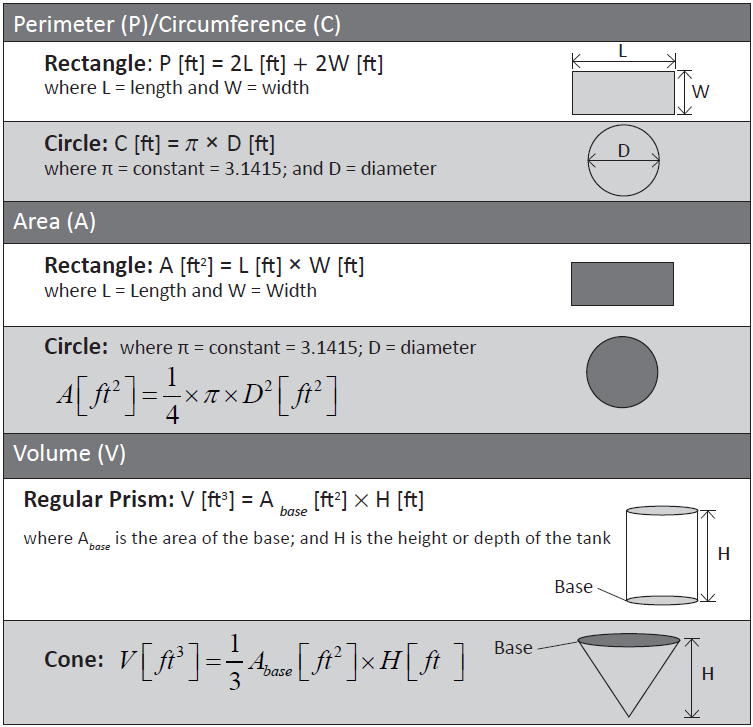
\includegraphics[scale=0.5]{Area&VolumeFormula}
\caption{Area and volume formulas}
\end{center}
\end{table}

\subsection{Example Problems}
% \hl{Example Problems}\\
\begin{enumerate}

\item The floor of a rectangular building is 20 feet long by 12 feet wide and the inside walls are 10 feet high. Find the total surface area of the inside walls of this building\\
Solution:\\
% \begin{center}
\begin{tikzpicture}
	%%% Edit the following coordinate to change the shape of your
	%%% cuboid
      
	%% Vanishing points for perspective handling
	\coordinate (P1) at (-7cm,1.5cm); % left vanishing point (To pick)
	\coordinate (P2) at (8cm,1.5cm); % right vanishing point (To pick)

	%% (A1) and (A2) defines the 2 central points of the cuboid
	\coordinate (A1) at (0em,0cm); % central top point (To pick)
	\coordinate (A2) at (0em,-2cm); % central bottom point (To pick)

	%% (A3) to (A8) are computed given a unique parameter (or 2) .8
	% You can vary .8 from 0 to 1 to change perspective on left side
	\coordinate (A3) at ($(P1)!.8!(A2)$); % To pick for perspective 
	\coordinate (A4) at ($(P1)!.8!(A1)$);

	% You can vary .8 from 0 to 1 to change perspective on right side
	\coordinate (A7) at ($(P2)!.7!(A2)$);
	\coordinate (A8) at ($(P2)!.7!(A1)$);

	%% Automatically compute the last 2 points with intersections
	\coordinate (A5) at
	  (intersection cs: first line={(A8) -- (P1)},
			    second line={(A4) -- (P2)});
	\coordinate (A6) at
	  (intersection cs: first line={(A7) -- (P1)}, 
			    second line={(A3) -- (P2)});

	%%% Depending of what you want to display, you can comment/edit
	%%% the following lines

	%% Possibly draw back faces

	\fill[gray!40] (A2) -- (A3) -- (A6) -- (A7) -- cycle; % face 6
	\node at (barycentric cs:A2=1,A3=1,A6=1,A7=1) {\tiny Floor=W*L};
	
	\fill[gray!50] (A3) -- (A4) -- (A5) -- (A6) -- cycle; % face 3
	\node at (barycentric cs:A3=1,A4=1,A5=1,A6=1) {\tiny Wall - W*H};
	
	\fill[gray!10, opacity=0.2] (A5) -- (A6) -- (A7) -- (A8) -- cycle; % face 4
	\node at (barycentric cs:A5=1,A6=1,A7=1,A8=1) {\tiny Wall - L*H};
	
	\fill[gray!10,opacity=0.5] (A1) -- (A2) -- (A3) -- (A4) -- cycle; % f2
	\node at (barycentric cs:A1=1,A2=1,A3=1,A4=1) {\tiny Wall - L*H};
	
	\fill[gray!40,opacity=0.2] (A1) -- (A4) -- (A5) -- (A8) -- cycle; % f5
	\node at (barycentric cs:A1=1,A4=1,A5=1,A8=1) {\tiny Ceiling=W*L};	
	
	\draw[thick,dashed] (A5) -- (A6);
	\draw[thick,dashed] (A3) -- (A6);
	\draw[thick,dashed] (A7) -- (A6);

	%% Possibly draw front faces

	%\fill[orange] (A1) -- (A8) -- (A7) -- (A2) -- cycle; % face 1
	\node at (barycentric cs:A1=1,A8=1,A7=1,A2=1) {\tiny Wall - W*H};
	


	%% Possibly draw front lines
	\draw[thick] (A1) -- (A2);

	\draw[<->] (-1.8,0.38) -- (-1.8,-1.3)node [midway, above=-1.8mm] {\hspace{-1.3cm}\tiny Height=10'};
	\draw[<->] (-1.6,-1.4) -- (-.3,-2.1)node [midway, above=-2.6mm] {\hspace{-1.3cm}\tiny Length=20'};
	\draw[<->] (2.6,-1.13) -- (0.2,-2.2)node [midway, below=.6mm] {\hspace{1.2cm}\tiny Width=12'};
	\draw[thick] (A3) -- (A4);
	\draw[thick] (A7) -- (A8);
	\draw[thick] (A1) -- (A4);
	\draw[thick] (A1) -- (A8);
	\draw[thick] (A2) -- (A3);
	\draw[thick] (A2) -- (A7);
	\draw[thick] (A4) -- (A5);
	\draw[thick] (A8) -- (A5);
	
	% Possibly draw points
	% (it can help you understand the cuboid structure)
%	\foreach \i in {1,2,...,8}
%	{
%	  \draw[fill=black] (A\i) circle (0.15em)
%	    node[above right] {\tiny \i};
%	}
	% \draw[fill=black] (P1) circle (0.1em) node[below] {\tiny p1};
	% \draw[fill=black] (P2) circle (0.1em) node[below] {\tiny p2};
\end{tikzpicture}\\
% \end{center}
2 Walls W*H + 2 Walls L*H= $2*12*10ft^2 + 2*20*10ft^2$\\
$=240+400=\boxed{640ft^2}$\\

2 Walls W*H + 2 Walls L*H + Floor + Ceiling= $2*12*10ft^2 + 2*20*10ft^2 + 2*12*20ft^2$\\
$=240+400+480=\boxed{1,120ft^2}$\\
\vspace{0.3cm}
\item How many gallons of paint will be required to paint the inside walls of a 40 ft long x 65 ft wide x 20 ft high tank if the paint coverage is 150 sq. ft per gallon.  Note:  We are painting walls only.  Disregard the floor and roof areas.\\
Solution:\\
\vspace{0.3cm}
% \begin{center}
\begin{tikzpicture}
	%%% Edit the following coordinate to change the shape of your
	%%% cuboid
      
	%% Vanishing points for perspective handling
	\coordinate (P1) at (-7cm,1.5cm); % left vanishing point (To pick)
	\coordinate (P2) at (8cm,1.5cm); % right vanishing point (To pick)

	%% (A1) and (A2) defines the 2 central points of the cuboid
	\coordinate (A1) at (0em,0cm); % central top point (To pick)
	\coordinate (A2) at (0em,-2cm); % central bottom point (To pick)

	%% (A3) to (A8) are computed given a unique parameter (or 2) .8
	% You can vary .8 from 0 to 1 to change perspective on left side
	\coordinate (A3) at ($(P1)!.8!(A2)$); % To pick for perspective 
	\coordinate (A4) at ($(P1)!.8!(A1)$);

	% You can vary .8 from 0 to 1 to change perspective on right side
	\coordinate (A7) at ($(P2)!.7!(A2)$);
	\coordinate (A8) at ($(P2)!.7!(A1)$);

	%% Automatically compute the last 2 points with intersections
	\coordinate (A5) at
	  (intersection cs: first line={(A8) -- (P1)},
			    second line={(A4) -- (P2)});
	\coordinate (A6) at
	  (intersection cs: first line={(A7) -- (P1)}, 
			    second line={(A3) -- (P2)});

	%%% Depending of what you want to display, you can comment/edit
	%%% the following lines

	%% Possibly draw back faces

	\fill[gray!40] (A2) -- (A3) -- (A6) -- (A7) -- cycle; % face 6
	\node at (barycentric cs:A2=1,A3=1,A6=1,A7=1) {};
	
	\fill[gray!50] (A3) -- (A4) -- (A5) -- (A6) -- cycle; % face 3
	\node at (barycentric cs:A3=1,A4=1,A5=1,A6=1) {\tiny Wall - W*H};
	
	\fill[gray!10, opacity=0.2] (A5) -- (A6) -- (A7) -- (A8) -- cycle; % face 4
	\node at (barycentric cs:A5=1,A6=1,A7=1,A8=1) {\tiny Wall - L*H};
	
	\fill[gray!10,opacity=0.5] (A1) -- (A2) -- (A3) -- (A4) -- cycle; % f2
	\node at (barycentric cs:A1=1,A2=1,A3=1,A4=1) {\tiny Wall - L*H};
	
	\fill[gray!40,opacity=0.2] (A1) -- (A4) -- (A5) -- (A8) -- cycle; % f5
	\node at (barycentric cs:A1=1,A4=1,A5=1,A8=1) {};	
	
	\draw[thick,dashed] (A5) -- (A6);
	\draw[thick,dashed] (A3) -- (A6);
	\draw[thick,dashed] (A7) -- (A6);

	%% Possibly draw front faces

	%\fill[orange] (A1) -- (A8) -- (A7) -- (A2) -- cycle; % face 1
	\node at (barycentric cs:A1=1,A8=1,A7=1,A2=1) {\tiny Wall - W*H};
	


	%% Possibly draw front lines
	\draw[thick] (A1) -- (A2);

	\draw[<->] (-1.8,0.38) -- (-1.8,-1.3)node [midway, above=-1.8mm] {\hspace{-1.3cm}\tiny Height=20'};
	\draw[<->] (-1.6,-1.4) -- (-.3,-2.1)node [midway, above=-2.6mm] {\hspace{-1.3cm}\tiny Length=45'};
	\draw[<->] (2.6,-1.13) -- (0.2,-2.2)node [midway, below=.6mm] {\hspace{1.2cm}\tiny Width=65'};
	\draw[thick] (A3) -- (A4);
	\draw[thick] (A7) -- (A8);
	\draw[thick] (A1) -- (A4);
	\draw[thick] (A1) -- (A8);
	\draw[thick] (A2) -- (A3);
	\draw[thick] (A2) -- (A7);
	\draw[thick] (A4) -- (A5);
	\draw[thick] (A8) -- (A5);
	
	% Possibly draw points
	% (it can help you understand the cuboid structure)
%	\foreach \i in {1,2,...,8}
%	{
%	  \draw[fill=black] (A\i) circle (0.15em)
%	    node[above right] {\tiny \i};
%	}
	% \draw[fill=black] (P1) circle (0.1em) node[below] {\tiny p1};
	% \draw[fill=black] (P2) circle (0.1em) node[below] {\tiny p2};
\end{tikzpicture}\\
% \end{center}
\vspace{0.3cm}
2 Walls W*H + 2 Walls L*H = $2*65*20ft^2 + 2*40*20ft^2= 2,600+1,600=4,200ft^2$\\
$\implies @150\dfrac{ft^2}{gal} \enspace paint \enspace coverage \enspace \rightarrow \enspace \dfrac{4,200\cancel{ft^2}}{150\dfrac{\cancel{ft^2}}{gal}}=\boxed{28 \enspace gallons}$
\vspace{0.3cm}
\item What is the circumference of a 100 ft diameter circular clarifier?\\
\vspace{0.3cm}
Solution:\\
\vspace{0.3cm}
$Circumference=\pi*D=3.14*100ft=\boxed{314ft}$
\vspace{0.3cm}
\item If the surface area of a clarifier is 5,025$ft^2$, what is its diameter?\\
\vspace{0.3cm}
Solution:\\
\vspace{0.3cm}
$Surface \enspace area=\dfrac{\pi}{4}*D^2 \enspace \implies 5025(ft^2)=0.785*D^2 (ft^2)$\\
$\implies D^2=\dfrac{5025}{0.785} \implies D=\sqrt{6401.3}=\boxed{80ft}$
\vspace{0.3cm}

\item How many gallons of wastewater would 600 feet of 6-inch diameter pipe hold, approximately?\\
\vspace{0.3cm}
Solution:\\

\vspace{0.3cm}
% \begin{center}
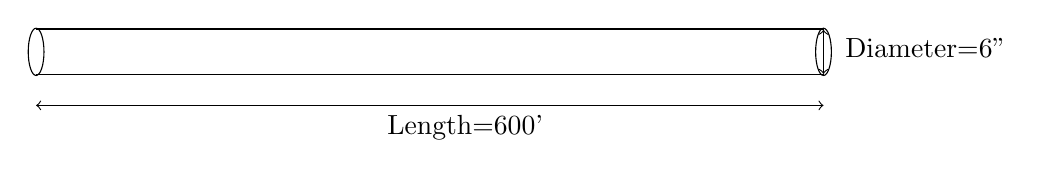
\begin{tikzpicture}
\draw (0,0) ellipse (0.1cm and 0.3cm);
\draw (10,0) ellipse (0.1cm and 0.3cm);
\draw [-] (0,-0.29) -- (10,-0.29);
\draw [-] (0,0.29) -- (10,0.29);
\draw [<->] (10,-0.28) -- (10,0.28) node [midway, below=-3mm] {\hspace{2.6cm}Diameter=6"};
\draw [<->] (0,-.68) -- (10,-.68)node [midway, below] {\hspace{0.9cm}Length=600'};
\end{tikzpicture}
% \end{center}
\vspace{0.3cm}
$Volume=\dfrac{\pi}{4}D^2*L=0.785*\Big(\dfrac{6}{12}\Big)^2*600\cancel{ft^3}*7.48\dfrac{gallons}{\cancel{ft^3}}=\boxed{881 \enspace gallons}$
\vspace{0.5cm}
\item A 110 ft diameter digester with a 12 ft deep cone is operated at a side water depth of 20 ft.  Caluclate the volume of sludge in the digester in $ft^3$ and gallons.\\
\vspace{0.3cm}
Solution:\\
\vspace{0.3cm}
% \begin{center}
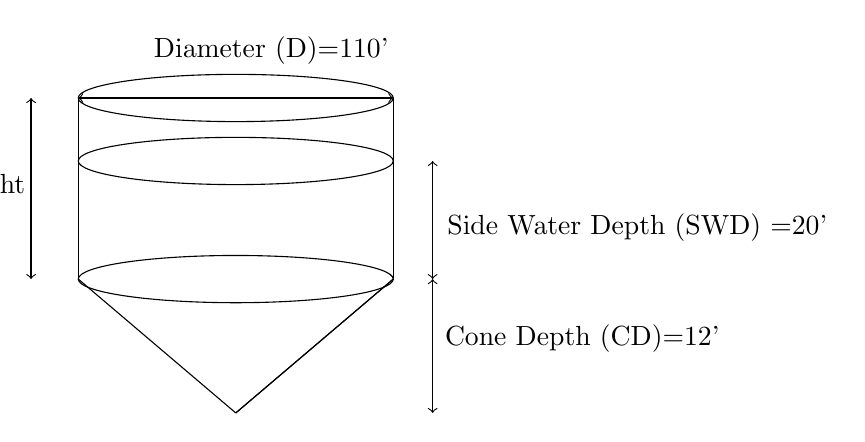
\begin{tikzpicture}
\draw (0,0) ellipse (2cm and 0.3cm);
\draw (0,-2.3) ellipse (2cm and 0.3cm);
\draw (0,-.8) ellipse (2cm and 0.3cm);
\draw [-] (2,-2.3) -- (2,0);
\draw [<->] (-2,0) -- (2,0) node [midway, below=-0.9cm] {\hspace{0.9cm}Diameter (D)=110'}; 
\draw [<->] (-2.6,-2.3) -- (-2.6,0) node [midway, below=-.3cm] {\hspace{-2.6cm}Cylinder Height};
\draw [<->] (2.5,-2.3) -- (2.5,-0.8) node [midway, below=-0.2cm] {\hspace{5.2cm}Side Water Depth (SWD) =20'};
\draw [-] (0,-4) -- (2,-2.3);
\draw [-] (0,-4) -- (-2,-2.3);
\draw [-] (0,-4) -- (2,-2.3);
\draw [-] (-2,0) -- (-2,-2.3);
\draw [<->] (2.5,-2.3) -- (2.5,-4)node [midway, below=-0.4cm] {\hspace{3.8cm}Cone Depth (CD)=12'};
\end{tikzpicture}\\
% \end{center}
$Digester \enspace volume=Volume_{cylinder}+Volume_{cone}$\\
$\implies Digester \enspace volume=\dfrac{\pi}{4}D^2*SWD+\dfrac{1}{3}*\Bigg(\dfrac{\pi}{4}*D^2*CD\Bigg)$\\
\vspace{0.3cm}
$=0.785*110^2*20+1.05*110^2*12=\boxed{227,988ft^3}$\\
\vspace{0.3cm}
$227,988\cancel{ft^3}*7.48\dfrac{gallons}{\cancel{ft^3}}=\boxed{1,705,352 \enspace gallons}$
\end{enumerate}

\section{Pounds Formula}



Pounds formula is used for:
\begin{itemize}
\item Calculating the quantity in pounds of a particular wastewater constituent entering or leaving a wastewater treatment process
\item Calculating the pounds of chemicals to be added\\
\end{itemize}
So if the concentration of a particular constituent (in mg/liter) and the volume or flow of wastewater is given, one can calculate the amount of that constituent in pounds using the following – Pounds Formula:
$$lbs \enspace \textbf{or} \enspace \dfrac{lbs}{day}=concentration(\dfrac{mg}{l})*8.34*volume(MG) \enspace \textbf{or} \enspace flow(\dfrac{MG}{day}(MGD)$$

\begin{figure}[h!]
\begin{center}
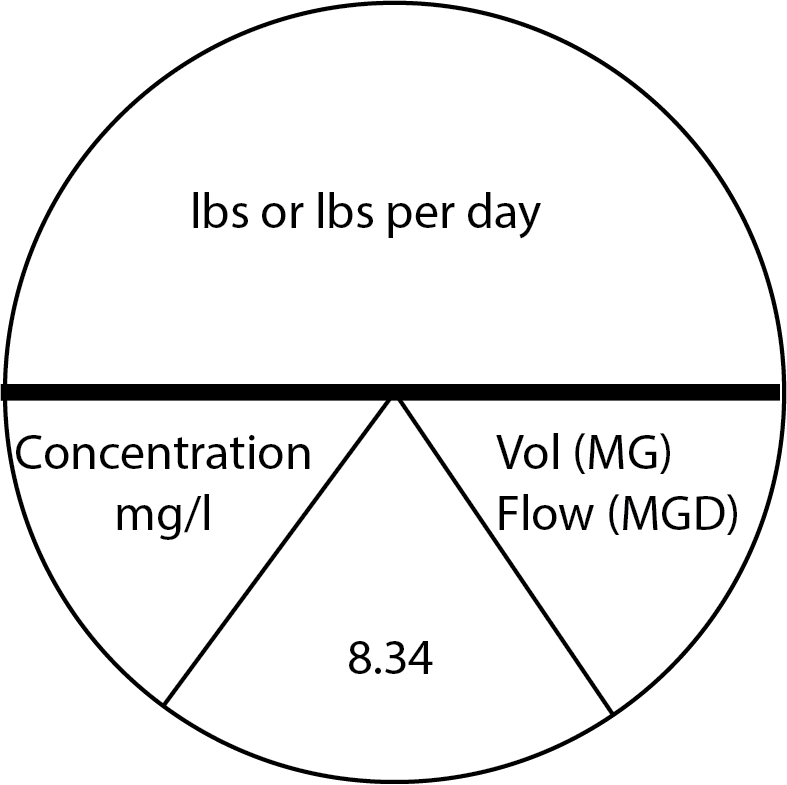
\includegraphics[scale=0.5]{PoundsFormula}
\end{center}
\caption{Pounds formula "nomograph"}
\end{figure}
\vspace{0.3cm}
There are three variables – (lbs, concentration and volume) and one constant (8.34) in the pounds formula.  Knowing any of the two variables in the formula, one can calculate the third (unknown) variable by rearranging the equation.


\newpage
\subsection{Concentration}\index{Concentration}

Concentration is typically expressed as mg/l which is the weight of the constituent (mg) in one  liter of solution (wastewater).  As one liter of water weighs one-million mg, a concentration of 1 mg/l implies 1 mg of constituent per 1 million mg of water or one part per million (ppm). \\ \textbf{Thus, mg/l and ppm are synonymous.}\\  
\vspace{6pt}
Sometimes the constituent concentration is expressed in terms of percentage.\\
\vspace{6pt}
For example:  sludge containing 5\% solids or a 12.5\% chlorine concentration solution.\\
\vspace{6pt}
As one liter of water weighs 1,000,000 mg, one percent of that weight is 10,000 mg.  \texthl{So 1\% solids implies 10,000 mg of solids per liter or 10,000 mg/l or 10,000 ppm.}\\
\vspace{6pt}
$1\%  \enspace concentration = 10,000 \enspace ppm \enspace or \enspace\dfrac{mg}{l}$\\
\vspace{4pt}
$0.1\% \enspace  concentration = 1,000 \enspace ppm \enspace or \enspace \dfrac{mg}{l}$\\
\vspace{4pt}
$0.01\% \enspace  concentration = 100 \enspace ppm \enspace or \enspace \dfrac{mg}{l}$\\
\vspace{4pt}
$10\% \enspace concentration = 100,000 \enspace ppm \enspace or \enspace \dfrac{mg}{l}$\\
\vspace{4pt}
$5\% \enspace  concentration = 50,000 \enspace ppm \enspace or \enspace \dfrac{mg}{l}$\\
\vspace{4pt}
$12.5\% \enspace  concentration = 125,000 \enspace ppm \enspace or \enspace \dfrac{mg}{l}$\\
\vspace{0.5cm}
\subsection{Example Problems}
% \hl{Example Problems}\\
\begin{enumerate}[1.]
\item Calculate the lbs/day of solids entering the plant given the influent flow is 5 MGD with an average solids concentration  of 250 mg/l.\\
\vspace{0.5cm}
Solution:\\
\vspace{0.5cm}
Applying lbs formula:\\
$\dfrac{lbs}{day}=5 MGD *250\dfrac{mg}{l}*8.34 = \boxed{10,425\dfrac{lbs}{day}}$
\\
\vspace{6pt}
\item Calculate the lbs of solids in the primary sludge if the sludge flow is 7500 gallons and the solids concentration is 4.5\%.\\
\vspace{0.5cm}
Solution:\\
\vspace{0.5cm}
Applying lbs formula:\\
\vspace{0.5cm}
$lbs \enspace solids = \dfrac{7500}{1,000,000}MG * 4.5*10,000 *8.34 = \boxed{2,815 \enspace lbs \enspace solids}$\\
\textbf{Note:}\\  
1) 7500 gallons was converted to MG by dividing by 1,000,000\\
\vspace{0.5cm}
$7500 \enspace gallons * \dfrac{1 MG}{1,000,000 \enspace gallon}$\\
\vspace{0.5cm}
2) 4.5\% was converted to mg/l by multiplying by 10,000 as 1\%=10,000mg/l
\end{enumerate}


\section{Process Removal Efficiency Calculations}\index{Process Removal Efficiency Calculations}

\begin{itemize}
\item Process removal rate or removal efficiency is the percentage of the inlet concentration removed.  
\item It is used for quantifying the pollutant removal during wastewater treatment and is established based upon the amount of a particular wastewater constituent entering and leaving a treatment process.

\item $Process \enspace Removal \enspace Rate \enspace (\%) = \dfrac{Pollutant \enspace  In-Pollutant\enspace  Out}{Pollutant \enspace In}*100$\\

\item If 10 units of a pollutant are entering a process and 8 units of pollutant are leaving (process removes 2 units), then the process removal rate for that pollutant is (10-8)/10*100=20\%.  In this example the process is 20\% efficient in removing that particular pollutant.

\item The amount of pollutant can be measured in terms of concentration (mg/l) or in terms of mass loading (lbs).  The pounds formula is used for calculating the mass loadings.  
\end{itemize}
The above example is for calculating the removal efficiency using the inlet and outlet concentrations or mass loading.\\
The methods below can be used for calculating either the inlet or outlet pollutant concentrations, if the removal efficiency and the corresponding inlet or outlet concentrations are given. 


\hl{Case 1:  Calculating outlet conc. (X) given the inlet conc. and removal efficiency (RE\%):}

\tikzstyle{block} = [rectangle, draw, fill=red!40, 
    text width=6em, text centered, rounded corners, minimum height=3em]
\tikzstyle{arrow} = [draw, -latex']
\begin{figure}[!h]
\centering
\begin{tikzpicture}[node distance =1.5cm, auto]
    \draw ++(0,0) node [block] (Process) {Process};
   \node[node distance=1.9in] (dummy_in) [left of=Process] {In};
   \node[node distance=1.9in] (dummy_out) [right of=Process] {Out};
	\node (Removal) [below of=Process, yshift=-0in] {$\tiny{Removal \enspace Efficiency=RE\% \enspace (Given)}$};
    \path [arrow] (dummy_in)-- (Process)  node [above] {\hspace{-5.8cm}$A \enspace mg/l \enspace (Given) $} node [below] {\hspace{-5.8cm}$100 \enspace mg/l$};
    \path [arrow] (Process) -- (dummy_out)  node [above] {\hspace{-4cm}$X \enspace mg/l \enspace (Unknown)$} node [below] {\hspace{-3.9cm}($100-RE\%)\enspace mg/l$};
   \draw[arrow] (Process) -- (Removal);
\end{tikzpicture}
\end{figure}
Using the fact that if the inlet concentration was 100 mg/l, the outlet concentration would be 100 minus the removal efficiency.\\
Setup the equation as:  $\dfrac{Out}{In}: \enspace \dfrac{X \enspace mg/l}{A \enspace mg/l}=\dfrac{100-RE\%}{100}$\\
Calculate X using cross multiplication - if $\dfrac{A}{B}=\dfrac{C}{D} \implies A=B*\dfrac{C}{D}$:\\
$X \enspace mg/l=A \enspace mg/l*\dfrac{100-RE\%}{100}$\\

\hl{Case 2:  Calculating inlet conc. (X) given the outlet conc. and removal efficiency (RE\%):}

\begin{figure}[!h]
\centering
\begin{tikzpicture}[node distance =1.5cm, auto]
    \draw ++(0,0) node [block] (Process) {Process};
   \node[node distance=1.9in] (dummy_in) [left of=Process] {In};
   \node[node distance=1.9in] (dummy_out) [right of=Process] {Out};
	\node (Removal) [below of=Process, yshift=-0in] {$Removal \enspace Efficiency=RE\% \enspace (Given)$};
    \path [arrow] (dummy_in)-- (Process)  node [above] {\hspace{-5.8cm}$X \enspace mg/l \enspace (Unknown)$} node [below] {\hspace{-5.8cm}$100 \enspace mg/l$};
    \path [arrow] (Process) -- (dummy_out)  node [above] {\hspace{-4cm}$A \enspace mg/l \enspace (Given)$} node [below] {\hspace{-3.9cm}($100-RE\%)\enspace mg/l$};
   \draw[arrow] (Process) -- (Removal);
\end{tikzpicture}
\end{figure}
Using the fact that if the inlet concentration was 100 mg/l, the outlet concentration would be 100 minus the removal efficiency.\\
Setup the equation as:  $\dfrac{In}{Out}: \enspace \dfrac{X \enspace mg/l}{A \enspace mg/l}=\dfrac{100}{100-RE\%}$\\
\vspace{0.3cm}
Calculate X using cross multiplication - if $\dfrac{A}{B}=\dfrac{C}{D} \implies A=B*\dfrac{C}{D}$:\\
$X \enspace mg/l=A \enspace mg/l*\dfrac{100}{100-RE\%}$\\

\vspace{0.4cm}
\hl{Example Problems:}\\

\begin{enumerate}

\item What is the \% removal efficiency if the influent concentration is 10 mg/L and the effluent concentration is 2.5 mg/L?\\
$Removal \enspace Rate (\%) = \dfrac{In-Out}{In}*100 \implies \dfrac{10-2.5}{10}*100=\boxed{75\%}$



\item Calculate the outlet concentration if the inlet concentration is 80 mg/l and the process removal efficiency is 60\%\\
Solution:\\

\tikzstyle{block} = [rectangle, draw, fill=red!40, 
    text width=6em, text centered, rounded corners, minimum height=3em]
\tikzstyle{arrow} = [draw, -latex']
\begin{figure}[!h]
\centering
\begin{tikzpicture}[node distance =1.5cm, auto]
    \draw ++(0,0) node [block] (Process) {Process};
   \node[node distance=1.5in] (dummy_in) [left of=Process] {In};
   \node[node distance=1.5in] (dummy_out) [right of=Process] {Out};
	\node (Removal) [below of=Process, yshift=-0in] {$Removal \enspace Efficiency=60\%$};
    \path [arrow] (dummy_in)-- (Process)  node [above] {\hspace{-4.39cm}$80mg/l$} node [below] {\hspace{-4.39cm}$100mg/l$};
    \path [arrow] (Process) -- (dummy_out)  node [above] {\hspace{-3.cm}$Xmg/l$} node [below] {\hspace{-3cm}40mg/l};
   \draw[arrow] (Process) -- (Removal);
\end{tikzpicture}
%\caption[MFCC]{Diagrama en bloques del cálculo de las MFCC para un frame.}
%\label{MFCC}
\end{figure}

$\dfrac{Out}{In} \enspace:\enspace\dfrac{Actual \enspace Outlet (X)}{80}=\dfrac{100-60}{100}$\\
$\implies \dfrac{Actual \enspace Outlet (X)}{80} =0.4$\\
$\implies Actual \enspace  Outlet (X) = 0.4 * 80 = \boxed{32 mg/l}$\\


\item Calculate the inlet concentration if the outlet concentration is 80 mg/l and the process removal efficiency is 60\%\\

\tikzstyle{block} = [rectangle, draw, fill=red!40, 
    text width=6em, text centered, rounded corners, minimum height=3em]
\tikzstyle{arrow} = [draw, -latex']
\begin{figure}[!h]
\centering
\begin{tikzpicture}[node distance =1.5cm, auto]
    \draw ++(0,0) node [block] (Process) {Process};
   \node[node distance=1.5in] (dummy_in) [left of=Process] {In};
   \node[node distance=1.5in] (dummy_out) [right of=Process] {Out};
	\node (Removal) [below of=Process, yshift=-0in] {$Removal \enspace Efficiency=60\%$};
    \path [arrow] (dummy_in)-- (Process)  node [above] {\hspace{-4.39cm}$Xmg/l$} node [below] {\hspace{-4.39cm}$100mg/l$};
    \path [arrow] (Process) -- (dummy_out)  node [above] {\hspace{-3.cm}80mg/l} node [below] {\hspace{-3cm}40mg/l};
   \draw[arrow] (Process) -- (Removal);
\end{tikzpicture}
\end{figure}

$\dfrac{In}{Out} \enspace : \enspace \dfrac{Actual \enspace inlet \enspace  (X)}{80}=\dfrac{100}{100-60}\implies \dfrac{Actual \enspace inlet \enspace  (X)}{80}=2.5$\\    
Rearranging the equation:   $Actual \enspace inlet (X)=2.5*80 = \boxed{200 mg/l}$\\

\item If a plant removes 35\% of the influent BOD in the primary treatment and 85\% of the remaining BOD in the secondary system, what is the BOD of the raw wastewater if the BOD of the final effluent is 20mg/l\\
Solution:\\

\begin{figure}[!h]
\centering
\begin{tikzpicture}[node distance =1.5cm, auto]
    \draw ++(0,0) node [block] (Primary) {Primary};
    
   \node[node distance=1.9in] (dummy_in) [left of=Primary] {Influent BOD};
   \node[node distance=1.9in] (dummy_out) [right of=Primary] {Primary BOD Out};
	\node (Removal) [below of=Primary, yshift=-0in] {$Removal \enspace Efficiency=35\% $};
    \path [arrow] (dummy_in)-- (Primary)  node [above] {\hspace{-4.8cm}$X \enspace mg/l \enspace$} node [below] {};
    \path [arrow] (Primary) -- (dummy_out)  node [above] {\hspace{-4.9cm}$0.65X \enspace mg/l$} node [below] {};
   \draw[arrow] (Process) -- (Removal);
\end{tikzpicture}
\end{figure}


\begin{figure}[!h]
\centering
\begin{tikzpicture}[node distance =1.5cm, auto]
    \draw ++(0,0) node [block] (Secondary) {Secondary};
    
   \node[node distance=1.9in] (dummy_in) [left of=Secondary] {Primary BOD Out};
   \node[node distance=1.9in] (dummy_out) [right of=Secondary] {Secondary BOD Out};
	\node (Removal) [below of=Secondary, yshift=-0in] {$Removal \enspace Efficiency=85\% $};
    \path [arrow] (dummy_in)-- (Secondary)  node [above] {\hspace{-4.8cm}$0.65X \enspace mg/l \enspace$} node [below] {\hspace{-5cm}$100 \enspace mg/l$};
    \path [arrow] (Secondary) -- (dummy_out)  node [above] {\hspace{-4.9cm}$20 \enspace mg/l$} node [below] {\hspace{-4.9cm}$15 \enspace mg/l$};
   \draw[arrow] (Process) -- (Removal);
\end{tikzpicture}
\end{figure}
\vspace{0.3cm}
For the Secondary process:\\
$\dfrac{In}{Out}: \enspace \dfrac{0.65X}{20}=\dfrac{100}{15} \implies X \enspace mg/l=\dfrac{100*20}{15*0.65}=\boxed{205 \enspace mg/l}$\\

\vspace{0.3cm}
Alternate Solution \#1

$\xrightarrow[
				\text{X}\dfrac{mg}{l}
			]
			{
			\text{Influent BOD}
			}
 \boxed{Primary}
 \xrightarrow[
 				\text{X-0.35X=X*(1-0.35)=0.65X}\dfrac{mg}{l}
 			]
 			{
 			\text{Primary Effluent BOD}
 			}
 \boxed{Secondary}
 \xrightarrow[
				\text{0.65X-0.5525X=(0.65-0.5525)X=0.0975X }
			 ]
			{
			\text{Secondary Effluent BOD}
			}
$\\
\hspace{2.8cm}$\downarrow$ {\tiny(0.35X)BOD Removed}\hspace{3.2cm}$\downarrow$ {\tiny(0.65*0.85)X = 0.5525X BOD Removed}\\
$\implies 0.0975X=20 \implies X=\dfrac{20}{0.0975}=\boxed{205\dfrac{mg}{l}}$\\

\vspace{0.3cm}

Alternate Solution \#2:\\
$\xrightarrow[\text{X}\dfrac{mg}{l}]{\text{Influent BOD}}\boxed{Primary}\xrightarrow[\text{0.65X}]{\text{Primary Effluent BOD}}\boxed{Secondary}\xrightarrow[\text{(0.65*0.15)X}]{\text{Secondary Effluent BOD}}$\\
\hspace{2.8cm}$\downarrow$ {\tiny(0.35X)BOD Removed}\hspace{2.2cm}$\downarrow$ {\tiny(0.65X*0.85)BOD Removed}\\

Primary Effluent BOD = Influent BOD * (1-Primary BOD Removal), and\\
Secondary Effluent BOD=[Primary Effluent BOD]*(1-Secondary BOD Removal)\\
Secondary Eff. BOD=[Influent BOD * (1-Primary BOD Removal)]*(1-Secondary BOD Removal)\\

Therefore, 20 = [X*(1-0.35)] * (1-0.85)= X*0.65*0.15\\
$\implies 20 \enspace \dfrac{mg}{l}= 0.0975X \implies X=\dfrac{20}{0.0975}=\boxed{205 \enspace \dfrac{mg}{l}}$\\

\end{enumerate}

\section{Preliminary Treatment Calculations}\index{Preliminary Treatment Calculations}

\subsection{Channel Velocity and Flow Rate}\index{Channel Velocity and Flow Rate}
Flow Rate - Q (volume/time) = velocity (distance or length traveled /time) * surface area\\
Velocity is the speed at which the water is flowing.  It is measured in units of length/time – ft./sec.\\
Velocity of water flowing through can be calculated by dividing the flow rate by area of the flow stream.\\
\vspace{0.5cm}
$Velocity \enspace \dfrac{length}{time}= \dfrac{flow \enspace rate(\dfrac{volume \enspace or \enspace cubic \enspace length}{time})}{surface \enspace area \enspace in \enspace the \enspace direction \enspace of \enspace flow-square \enspace length}$\\
\newpage
\textbf{For a flow in a channel:}\\
\vspace{0.5cm}
\hl{Example Problems:}\\
\begin{enumerate}[1.]
\item Calculate the velocity of a 14 MGD flow in a 6 ft wide channel with a water depth of two feet.\\
\begin{center}
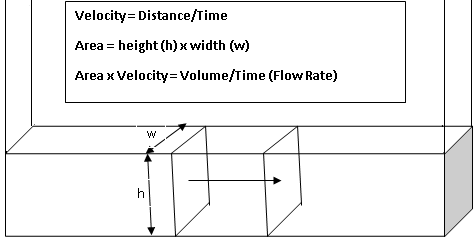
\includegraphics[scale=0.5]{ChannelFlow3}
\end{center}
$Flow (Q) = Velocity (V) * Area (A)$\\
$\implies 14 \dfrac{MG}{day}* \dfrac{10^6 gal}{MG} * \dfrac{ft^3}{7.48 gal}*\dfrac{day}{24*60*60} = V \dfrac{ft}{sec}* 6 ft * 2 ft \implies 21.7 \dfrac{ft^3}{sec}= 12V\dfrac{ft^3}{sec}$\\
$\implies V \dfrac{ft}{sec}= \dfrac{21.7}{12}= \boxed{1.8\dfrac{ft}{sec}}$\\

\item Calculate the flow, in gpd, that would pass through a grit chamber 2 feet wide, at a depth of 6 inches, with a velocity of 1 ft /sec\\
Solution:\\
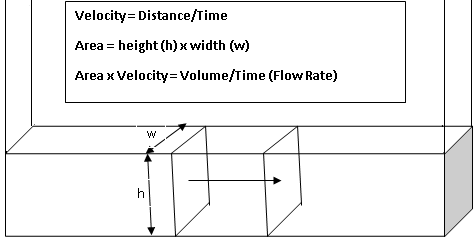
\includegraphics[scale=0.5]{ChannelFlow3}\\
$Q=V*A$\\
$Q=1\dfrac{ft}{s}*(2*0.5)ft^2=1\dfrac{ft^3}{s}$\\
$Q=1\dfrac{\cancel{ft^3}}{\cancel{s}}*\dfrac{(1440*60)\cancel{s}}{day}*7.48\dfrac{gal}{\cancel{ft^3}}=\boxed{646,272\dfrac{gal}{day}}$
\vspace{0.5cm}
\item A wastewater channel is 3.25 feet wide and is conveying a wastewater flow of 3.5 MGD. The wastewater flow is 8 inches deep. Calculate the velocity of this flow.\\
Solution:\\
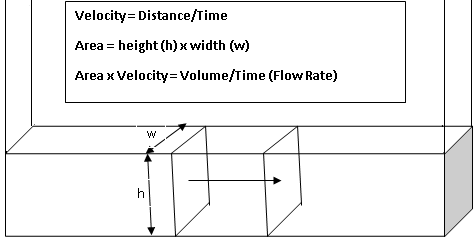
\includegraphics[scale=0.5]{ChannelFlow3}\\
$Q=V*A \implies V=\dfrac{Q}{A}$\\
$\implies V\dfrac{ft}{s}=\dfrac{3.5\dfrac{\cancel{MG}}{\cancel{day}}*\dfrac{1000000\cancel{gal}}{\cancel{MG}}*\dfrac{ft^{\cancel{3}}}{7.48\cancel{gal}}*\dfrac{\cancel{day}}{(1440*60)s}}{(3.25*0.75)\cancel{ft^2}}=\boxed{2.2\dfrac{ft}{s}}$
\vspace{0.5cm}
\item A plastic float is dropped into a wastewater channel and is found to travel 10 feet in 4.2 seconds. The channel is 2.4 feet wide and is flowing 1.8 feet deep. Calculate the flow rate of this wastewater in cubic feet per second.\\
Solution:\\
$Q=V*A$\\
$\implies Q\Big(\dfrac{ft^3}{s}\Big)=\dfrac{10ft}{4.2s}*(2.4*1.8)ft^2=\boxed{10.3\dfrac{ft^3}{s}}$
\end{enumerate}

\subsection{Grit Removal Rates}\index{Grit Removal Rates}
\emph{Typical grit removal ranges from 0.5 to 30 ft$^3$/MG}\\
\vspace{0.3cm}
\hl{Example Problems:}\\
\begin{enumerate}[1.]
\item At a wastewater treatment plant which receives a flow rate of 650,000 gallons per day, a total of 50 cubic feet of grit was removed for the month. Calculate the rate of grit removal assuming 30 days in a month.\\
Solution:\\
$Grit Removal\dfrac{ft^3}{MG}=50\dfrac{ft^3}{ \cancel{month}}*\dfrac{\cancel{month}}{30\cancel{days}}*\dfrac{\cancel{day}}{650,000\cancel{gal}}*1,000,000\dfrac{\cancel{gal}}{MG}=\boxed{2.6\dfrac{ft^3}{MG}}$
\end{enumerate}

\section{Primary Treatment Calculations}\index{Primary Treatment Calculations}

\subsection{Hydraulic or Surface Loading Rate}\index{Hydraulic or Surface Loading Rate}

The hydraulic or surface loading rate measures how rapidly wastewater moves through the primary clarifier.  It is measured in terms of the number of gallons flowing each day through one square foot surface area of the clarifier. 
$$Clarifier \enspace hydraulic \enspace loading \enspace 	\Big(\dfrac{gpd}{ft^2}\Big) =\dfrac{Clarifier \enspace influent 	\enspace flow (gpd)}{Clarifier \enspace surface \enspace area 	(ft^2)}$$ 
		Rectangular clarifier surface area  = width * length\\
		Circular clarifier surface area  = 0.785 * Diameter$^2 $\\
\subsection{Detention Time}\index{Detention Time}

Detention time is the length of time that wastewater stays in the settling tank is called the detention time.  It is also the time it takes for a unit volume of wastewater to pass entirely through a primary clarifier\\
$$Clarifier \enspace detention \enspace time \enspace (hr) = 	\dfrac{ Clarifier \enspace volume (cu.ft \enspace or \enspace gal)}{Influent \enspace flow \enspace (cu.ft \enspace or \enspace gal)/hr)}$$
Rectangular clarifier volume = width * length * depth of water\\
Circular clarifier volume = 0.785 * Diameter$^2$ * depth of water\\
Typically volume is calculated in cu. ft and influent flow is given in gallons.  Use 7.48 gal/ft$^3$ conversion factor to convert volume in cu. ft to gallons.\\

\subsection{Weir Overflow Rate}\index{Weir Overflow Rate}
The weirs at the end of the primary clarifier allow for the even distribution of the the outlet flow across the entire length of the weir.  An adequate length of weir is needed to ensure smooth and even flow of wastewater over the weirs.  Weir overflow rate measures the number of gallons of wastewater per day flowing over one foot of weir. 

		$$Weir \enspace over \enspace flow \enspace rate \Big(\dfrac{gpd}{ft}\Big) =\Big(\dfrac{Clarifier \enspace influent \enspace  flow (gpd)}{Total \enspace effluent 					\enspace weir \enspace length \enspace (ft)}\Big)$$
		Circular clarifier weir length = 3.14 * Diameter\\

\hl{Example problem for (a), (b) and (c) above:}\\
		\vspace{0.2cm}
A circular clarifier receives a flow of 11 MGD.  If the clarifier is 90 ft. in diameter and is 12 ft. deep, what is: a) the hydraulic/surface loading rate, b) clarifier detention time in hours, and c) weir overflow rate?\\
		\vspace{0.2cm}
a) Hydraulic/surface loading rate:\\
$Clarifier \enspace hydraulic \enspace loading \enspace 	\Big(\dfrac{gpd}{ft^2}\Big) ==\dfrac{\dfrac{11\cancel{MG}}{{day}}*\dfrac{10^6gal}{\cancel{MG}}}{0.785*90^2 ft^2}=\boxed{1,730gpd/ft^2}$\\
		\vspace{0.5cm}
b) Clarifier detention time:\\
$Clarifier \enspace detention \enspace time \enspace (hr) = 	\dfrac{ Clarifier \enspace volume (cu.ft \enspace or \enspace gal)}{Influent \enspace flow \enspace (cu.ft \enspace or \enspace gal)/hr)}$\\
		\vspace{0.2cm}
$Clarifier \enspace detention \enspace time \enspace (hr) = 	\dfrac{(0.785*90^2*15)\cancel{ft^3}}{\dfrac{11\cancel{MG}}{\cancel{day}}*\dfrac{10^6\cancel{gal}}{\cancel{MG}}*\dfrac{\cancel{ft^3}}{7.48\cancel{gal}}*\dfrac{\cancel{day}}{24hrs}}=\boxed{2hrs}$\\
		\vspace{0.5cm}
c) Weir overflow rate:\\
		\vspace{0.2cm} 
$Weir \enspace overflow \enspace rate \Big(\dfrac{gpd}{ft}\Big) =\dfrac{\dfrac{11\cancel{MG}}{{day}}*\dfrac{10^6gal}{\cancel{MG}}}{3.14*90 ft}=\boxed{38,924gpd/ft}$\\

\subsection{Removal Efficiency}\index{Removal Efficiency}		
Primary sedimentation removes suspended wastewater solids which includes BOD.  The efficiency of the primary is established as the percentage of the amount of parameter removed.  The parameter may quantified as mass (lbs) or as concentration (mg/l).

$$Removal \enspace efficiency (\%) = \dfrac{Parameter  \enspace In - Parameter  \enspace Out}{Parameter \enspace In} * 100$$

For TSS removal:\\
$$TSS \enspace Removal \enspace efficiency (\%) = \dfrac{TSS  _{In} \enspace(mg/l)  - TSS_{Out} \enspace(mg/l)  }{TSS _{In} \enspace(mg/l)  } * 100$$

For BOD removal:\\
$$BOD \enspace Removal \enspace efficiency (\%) = \dfrac{BOD_{In} \enspace(mg/l)  - BOD_{Out} \enspace(mg/l)  }{BOD _{In} \enspace(mg/l)  } * 100$$
\subsection{Solids Removal}\index{Solids Removal}	

\hl{\textbf{Type 1 Problems:}  These involve calculating lbs of solids removed given any two of the following TSS parameters - inlet concentration, outlet concentration and removal efficiency.}\\
a. If the inlet and outlet concentrations are given, calculate the mg/l of TSS removed using: 
$$TSS_{removed} = TSS_{in}(mg/l) - TSS_{out} (mg/l) $$
Then knowing the flow, use the lbs formula to calculate the lbs solids removed.

b. If either inlet or outlet concentration is given along with the clarifier removal efficiency, using the removal efficiency calculate the unknown outlet concentration (if only the inlet is given) or the inlet concentration (if only the outlet is given)\\
i) If inlet and removal efficiency is given, calculate the outlet by subtracting the product of inlet and removal efficiency from the inlet.
$$TSS_{out}=TSS_{in} - (TSS_{in}*\%Removal)$$
Example if the removal efficiency is 60\% and the inlet concentration is 300mg/l: $$TSS_{out}=300 - 300*0.6=120mg/l$$
ii) If outlet and removal efficiency is given, calculate the inlet concentration by dividing the outlet by (1-removal efficiency).\\
$$TSS_{in}=\dfrac{TSS_{out}}{1-\%Removal}$$
Example if the removal efficiency is 60\% and the outlet concentration is 120mg/l: $$TSS_{in}=\dfrac{120}{1-0.6}=300mg/l$$ 

Note:  You may derive the above formulas by algebraically manipulating: $\%Removal=\dfrac{TSS_{in} -TSS_{out}}{TSS_{in}}$\\
\hl{Example Problem:}\\
How many lbs of solids are removed daily by a primary clarifier treating a 6 MGD flow if the average influent TSS concentration is 300 mg/l and the clarifier TSS removal efficiency is 67\%.\\
$TSS_{out}=(300mg/l - 300*0.67)=99mg/l$\\
$lbs \enspace solids \enspace  removed = (300-99)mg/l*8.34*6MGD=\boxed{10,058 \enspace lbs \enspace solids \enspace removed \enspace per \enspace day}$\\
\vspace{0.5cm}
\hl{\textbf{Type 2 Problems:}  These involve calculating the amount of sludge pumping given the solids removed.  The solids removed from the primary clarifier is sludge with a typical solids concentration of about 3\% to 5\%.}\\
Given the amount of total solids removed and given the sludge concentration, the volume of sludge pumping can be calculated as follows:  $$\dfrac{ft^3\enspace sludge\enspace pumped}{ day}= \dfrac{lbs \enspace solids \enspace (removed)}{day} * \dfrac{1 \enspace lb \enspace sludge}{(\%)\enspace lbs \enspace solids}*\dfrac{gal \enspace sludge}{8.34lb \enspace sludge}*\dfrac{ft^3 \enspace sludge}{7.48 \enspace gal} $$
So for the solids removed in the above example, if the primary sludge has 5\% solids, the required sludge pumping can be calculated as:
$$\dfrac{ft^3\enspace sludge}{day}= \dfrac{10,058 \enspace \cancel{lbs \enspace solids}}{day} * \dfrac{1 \enspace \cancel{lb \enspace sludge}}{0.05\enspace \cancel{lbs \enspace solids}}*\dfrac{\cancel{gal \enspace sludge}}{8.34\cancel{lb \enspace sludge}}*\dfrac{ft^3 \enspace sludge}{7.48 \enspace \cancel{gal}}=\boxed{3,224\dfrac{ft^3 \enspace sludge}{day}} $$
